\documentclass{article}
\usepackage{graphicx}
\usepackage{amsmath}
\usepackage{pgfplots}
\usepackage{physics}
\usepackage{cancel}
\usepackage{enumitem}
\usepackage{txfonts}

\pgfplotsset{compat=1.18}

\usepackage[a4paper, top=1cm, bottom=2cm, left=2cm, right=2cm, includehead, includefoot]{geometry}

\begin{document}

\noindent
Physics 4A - Classical Mechanics \hfill Prof. Roger King

\noindent\rule{\textwidth}{0.4pt}

\begin{center}
    \textbf{\LARGE Homework 3} \\
    \vspace{12pt}
    \large Aaron W. Tarajos \\
    \textit{\today}
\end{center}

\noindent\rule{\textwidth}{0.4pt}

\section*{Problem 1}
Given the three vectors $\va A = 1.00 \vu i  -4.00 \vu j$, $\va B = 3.00 \vu i$, and $\va C = -2.00 \vu j$ evaluate the following expressions if they are allowed mathematically: (a) $\va C \cdot \left( \va A + \va B \right)$; (b) $\va C \cdot \left( \va A \cdot \va B \right)$; (c) $C + \va A \cdot \va B$.

\subsection*{Solution}
\subsubsection*{Part a:}
\begin{align*}
	\va C \cdot \left( \va A + \va B \right) &= \va C \cdot \left((1.00 \vu i  -4.00 \vu j) + (3.00 \vu i)\right) \\
	&= (0.00 \vu i -2.00 \vu j) \cdot \left( 4.00 \vu i -4.00 \vu j\right) \\
	&= 0.00 + 8.00 \\
	&= 8.00
\end{align*}

\subsubsection*{Part b:}
The expression is not mathematicall valid because the dot product of $\va A$ and $\va B$ will always be a scalar and you cannot take the dot product of a scalar and a vector.

\subsubsection*{Part c:}
\begin{align*}
	\va C + \va A \cdot \va B &= 2.00 + (1.00 \vu i  -4.00 \vu j) \cdot (3.00 \vu i + 0.00 \vu j) \\
				  &= 2.00 + 3.00 + 0.00 \\
				  &= 5.00
\end{align*}

\section*{Problem 2}
Given three vectors, $\va A = 2.00 \vu i - 5.00 \vu j$, $\va B = 4.00 \vu j$, and $\va C = 3.00 \vu i$, evaluate the following expressions if they are mathematically allowed:
(a) $C \left( \va A \cross \va B \right)$;
(b) $\va C \cdot \left(\va A \cross \va B \right)$;
(c) $\va C \cross \left(\va A \cdot \va B \right)$.

\subsection*{Solution}
\subsubsection*{Part a:}
\begin{align*}
	C \left( \va A \cross \va B \right) &= 3.00 * \det \left( \mqty[\vu i & \vu j & \vu k \\ 2.00 & -5.00 & 0.00 \\ 0.00 & 4.00 & 0.00] \right) \\
					    &= 3.00 \left( \mqty[-5.00 & 0.00 \\ 4.00 & 0.00]\ \vu i - \mqty[2.00 & 0.00 \\ 0.00 & 0.00]\ \vu j + \mqty[2.00 & -5.00 \\ 0.00 & 4.00]\ \vu k \right) \\
					    &= 3.00 \left( 0.00 \vu i - 0.00 \vu j + 8.00 \vu k \right) \\
					    &= 24.00 \vu k
\end{align*}

\subsubsection*{Part b:}
We already know that $\va A \cross \va B$ is $\left( 0.00 \vu i - 0.00 \vu j + 8.00 \vu k \right)$, therefore;
\begin{align*}
	\va C \cdot \left(\va A \cross \va B \right) &= \left( 3.00 \vu i + 0.00 \vu j + 0.00 \vu k \right) \cdot \left( 0.00 \vu i - 0.00 \vu j + 8.00 \vu k \right) \\
						     &= 0.00 + 0.00 + 0.00 \\
						     &= 0.00
\end{align*}

\subsubsection*{Part c:}
The expression is not mathematically valid  because $\va A \cdot \va B$ is a scalar and you cannot take the cross product of a vector and a scalar.

\section*{Problem 3}
Consider two vectors $\va A$ and $\va B$ where:
\begin{align*}
	\va A &= -6.00 \vu i + 3.00 \vu j + 3.00 \vu k \\
	\va B &= 6.00 \vu i -8.00 \vu j + 4.00 \vu k
\end{align*}
If we want to find the angle between these two vectors, we have two possible options: we can use the magnitude of the dot product, or the magnitude of the cross product.
\[
	\va A \cdot \va B = AB \cos\theta
\]
\[
	\left| \va A \cross \va B \right| = AB \sin\theta
\]
However, these approaches give conflicting answers for the value of $\theta$. \\
(a) What is the correct value of theta? \\
(b) Why does the other formula give the wrong answer?

\subsection*{Solution}
The dot product gives the correct value of theta;
\begin{align*}
	\va A \cdot \va B &= AB \cos\theta \\
	\frac{\va A \cdot \va B}{AB} &= \cos\theta \\
	\theta &= \arccos\left( \frac{\va A \cdot \va B}{AB} \right)
\end{align*}
Then we plugin our values,
\[
	\arccos\left( \frac{\left( -36.00 - 24.00 + 12.00  \right)}{\sqrt{-6.00^2 + 3.00^2 + 3.00^2} \sqrt{6.00^2 -8.00^2 + 4.00^2}} \right) = 127.34^\circ \quad .
\]
The reason that the cross product method is wrong in this situation is because the smaller angle between $\va A$ and $\va B$ is not theta relative to the origin so the actual angle for the cross product method should be $\sin(360 - \theta)$.

\section*{Problem 4}
The position of an object as a function of time is given by $r\left(t \right) = \left( 3.00t^2 - 2.00t \right)\vu i - 1.00t^3 \vu j$ m. Find (a) its velocity at $t=2.00$ s; (b) its acceleration at $t=4.00$ s; (c) its average acceleration between $t=1.00$ s and $t=3.00$ s.

\subsection*{Solution}
\subsubsection*{Part a:}
Velocity is the derivative of position with respect to time so we differentiate the position function and evaluate it at $t=2.00$;
\begin{align*}
	r^\prime \left( t \right) &= \left(6.00 t - 2.00 \right)\ \vu i - 3.00t^2\ \vu j \\
	r^\prime \left( 2 \right) &= \left(6.00 (2.00) - 2.00 \right)\ \vu i - 3.00(2.00)^2\ \vu j \\
				  &= 10.00\ \vu i - 12.00\ \vu j
\end{align*}
\subsubsection*{Part b:}
Similarly, acceleration is the derivative of velocity with respect to time so we differentiate the velocity function and evaluate it at $t=4.00$
\begin{align*}
	r^{\prime\prime} \left( t \right) &= \left(6.00\right)\ \vu i - 6.00t\ \vu j \\
	r^{\prime\prime} \left( 4 \right) &= \left(6.00\right)\ \vu i - 6.00(4.00)\ \vu j \\
				  &= 6.00\ \vu i - 24.00\ \vu j
\end{align*}

\subsubsection*{Part c:}
To find the average velocity we evaluate the velocity at the respective times and take the difference over change in time.
\[
	\va v_1 = (6.00(1.00) - 2.00)\ \vu i - 3.00(1.00^2)\ \vu j  = 4.00\ \vu i - 3.00\ \vu j
\]
\[
	\va v_2 = (6.00(3.00) - 2.00)\ \vu i - 3.00(3.00^2)\ \vu j = 16.00\ \vu i - 27.00\ \vu j
\]
Then
\[
	\frac{\left( 16.00\ \vu i - 27.00\ \vu j \right) - \left( 4.00\ \vu i - 3.00\ \vu j \right)}{2.00} = 6.00\ \vu i -12.00\ \vu j
\]

\section*{Problem 5}
At $t = 0$ a particle at the origin has a velocity of $15.1$ m/s at $36^\circ$ above the horizontal $x$ axis.
At $t = 5.00$ s it is at $x = 21.0$ m and $y = 35.0$ m and its velocity is 30.0 m/s at $53^\circ$ above the horizontal.
Find: (a) its average velocity; (b) its average acceleration.

\subsection*{Solution}
\subsubsection*{Part a:}
We know the components of the position vector for $t = 5$ and because we start at the origin the average velocity is simply the difference in the position over time.
\begin{align*}
	\va v_{avg} &= \frac{\left( 21.0\ \vu i + 35.0\ \vu j \right) - \left( 0\ \vu i + 0\ \vu j \right)}{5 - 0} \\
		  &= 4.2 \vu i + 7 \vu j
\end{align*}

\subsubsection*{Part b:}
To find the average acceleration we start by converting the respective velocities to unit vector notation and then take the difference over time.
\begin{align*}
	\va a_{avg} &= \frac{\left(30.0 \cos(53)\ \vu i + 30.0 \sin (53)\ \vu j \right) - \left(15.1 \cos(36)\ \vu i + 15.1 \sin (36)\ \vu j\right)}{5}\\
		    &= \frac{\left( 18.0545\ \vu i + 23.9591\ \vu j\right) - \left(12.2162\ \vu i + 8.8756\ \vu j \right)}{5} \\
		    &= 1.168\ \vu i + 3.017\ \vu j
\end{align*}

\section*{Problem 6}
Personnel at an airport control tower track a UFO. At 11:02 a.m. it is located at a horizontal distance of 2.00 km in the direction $30^\circ$ N of E at an altitude of 1200 m.
At 11:15a.m. the location is 1.00 km at $45^\circ$ S of E at an altitude of 800 m.
What was the displacement of the UFO? Express your result in component notation.
\begin{figure}[ht]
    \centering
    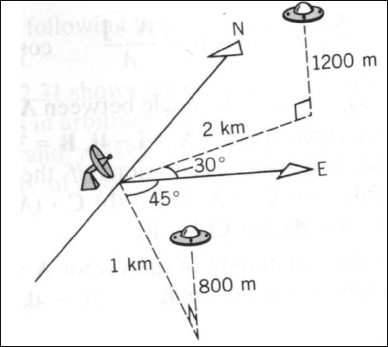
\includegraphics[scale=0.5]{drawing-1.png}
\end{figure}

\subsection*{Solution}
The $\vu k$ component of the initial position vector is given so we just need to find the $\vu i$ and $\vu j$ components.
\begin{align*}
	\va x_0 &= 2\cos(30)\ \vu i + 2\sin(30)\ \vu j + 1200\ \vu k \\
		&= 1.7321\ \vu i + 1\ \vu j + 1200\ \vu k \quad \text{m}
\end{align*}
Then the final position vector is
\begin{align*}
	\va x &= \cos(-45)\ \vu i + \sin(-45)\ \vu j + 800\ \vu k \\
	      &= 0.7071\ \vu i -0.7071\ \vu j + 800\ \vu k \quad \text{m}
\end{align*}
The displacement is the difference between final position and the initial position;
\begin{align*}
	\Delta \va x &= \left(0.7071\ \vu i -0.7071\ \vu j + 800\ \vu k \right) - \left( 1.7321\ \vu i + 1\ \vu j + 1200\ \vu k \right) \\
		     &= -1.025\ \vu  i - 1.7071\ \vu j -400\ \vu k
\end{align*}

\section*{Problem 7}
A fastball pitcher can throw a baseball at a speed of 90.0 mi/h.
(a) Assuming the pitcher can release the ball 16.7 m from home plate so the ball is moving horizontally, how long does it take
the ball to reach home plate?
(b) How far does the ball drop between the pitcher’s hand and home plate?

\subsection*{Solution}
The speed of 90.0 mi/h is 40.2336 m/s so we find that the ball took;
\[
	\frac{16.7\ \text{m}}{40.2336 \text{m/s}} = 0.415\ \text{s} \quad .
\]
The drop of the ball is given by;

\begin{equation}
	\Delta x =  v_0 t + \frac{1}{2}gt^2
\end{equation}
where $g$ is the acceleration of gravity near the earth's surface. The initial downward velocity is zero, therefore the ball drops;
\begin{align*}
	\Delta x &= (0)(0.415) + \frac{1}{2}9.81(0.415)^2 \\
		 &= \frac{1.6895}{2} \\
		 &= 0.845\ \text{m}
\end{align*}

\section*{Problem 8}
A soccer goal is 2.44 m high. A player kicks the ball at a distance 10.0 m from the goal at an angle of $25.0^\circ$.
The ball hits the crossbar at the top of the goal.
What is the initial speed of the soccer ball?

\subsection*{Solution}
The initial velocity $\va v_{0}$ is going to be
\begin{align*}
	\va v_0 &= v_{0x}\ \vu i + v_{0y}\ \vu j \\
		&= v_0 \cos \theta\ \vu i + v_0 \sin\theta\ \vu j \\
		&= v_0\cos(25)\ \vu i + v_0\sin(35)\ \vu j \\
		&= 0.906 v_0\ \vu i + 0.423 v_0\ \vu j
\end{align*}
and so we have to solve for the magnitude of $\va v_0$. Using
\begin{equation*}
	\Delta x = v_{0x} t + \frac{1}{2}a_x t
\end{equation*}
we have
\begin{align*}
	10.00 &= 0.906 v_0t + \frac{1}{2}(0) t^2 \\
	v_0t &= 11.0378 t
\end{align*}
Now that we solved for $v_0t$ we can use the vertical dispalcement with the same equation to find time;

\end{document}
